% Fuente: Pauta del Control 2, Pregunta 1.
\begin{enumerate}
  \item[(a)]
 
\[
\max\; z = 5x_1+4x_2 \qquad
\text{s.a.}\quad
\begin{cases}
6x_1+4x_2 \le 24 & \text{(protecciones)}\\
x_1+2x_2 \le 6 & \text{(tablero)}\\
x_1,x_2 \ge 0,\ \text{enteros.}
\end{cases}
\]
 
\textbf{Relajaci\'on lineal.} Quitando la integralidad, los v\'ertices de la regi\'on factible son
\begin{equation}
    (0,0),\:(4,0),\:(0,3)
\end{equation}
y la intersecci\'on de ambas restricciones. Resolviendo
$6x_1+4x_2=24$ con $x_1+2x_2=6$ se obtiene $x_2=\tfrac32,\ x_1=3$. Evaluando $z$:
\[
(4,0)\to 20,\quad (0,3)\to 12,\quad \Big(3,\tfrac32\Big)\to 21.
\]
El \'optimo de la relajaci\'on es $\big(3,\tfrac32\big)$ con $\boxed{z^*_{LP}=21}$ (fraccionario en $x_2$).
 
\textbf{Envoltura convexa.} El cierre convexo de los puntos enteros factibles tiene v\'ertices
$(0,0),(4,0),(2,2),(0,3)$, basta con añadir la recta $x_1+x_2\le 4$:

\begin{center}
\begin{tikzpicture}[scale=1.35]
  \fill[gray!16]  (0,0) -- (4,0) -- (3,1.5) -- (0,3) -- cycle;
  \fill[blue!14]  (0,0) -- (4,0) -- (2,2)   -- (0,3) -- cycle;
  \draw[step=1,gray!30,very thin] (0,0) grid (4.5,3.5);
  \draw[->] (0,0) -- (4.9,0) node[right]{$x_1$};
  \draw[->] (0,0) -- (0,3.8) node[above]{$x_2$};
  \foreach \x in {1,2,3,4} \draw (\x,0.04)--(\x,-0.04) node[below]{\footnotesize\x};
  \foreach \y in {1,2,3} \draw (0.04,\y)--(-0.04,\y) node[left]{\footnotesize\y};
  % restricciones
  \draw[orange!75!black,thick] (4,0) -- (1.667,3.5) node[pos=0.85,left]{\footnotesize $6x_1{+}4x_2\le24$};
  \draw[teal!70!black,thick]   (0,3) -- (4.5,0.75) node[pos=0.92,below]{\footnotesize $x_1{+}2x_2\le6$};
  % faceta entera
  \draw[blue!70!black,very thick] (4,0) -- (2,2) node[midway,below left,blue!60!black]{\footnotesize $x_1{+}x_2\le4$};
  % puntos enteros
  \foreach \p in {(0,0),(1,0),(2,0),(3,0),(4,0),(0,1),(1,1),(2,1),(3,1),(0,2),(1,2),(2,2),(0,3)}
    \fill \p circle (1.5pt);
  % optimo relajacion
  \draw[red!75!black,thick] (3,1.5) circle (3.2pt);
  \node[red!70!black,above right,inner sep=1pt] at (3,1.5) {\footnotesize $(3,\tfrac32)$, $z{=}21$};
  % optimo entero
  \fill[green!55!black] (4,0) circle[radius=2.2pt];
  \node[green!45!black,above right,inner sep=1pt] at (4,0.05) {\footnotesize $(4,0)$, $z{=}20$};
\end{tikzpicture}
\end{center}
 
  \item[(b)]
 
Basta a\~nadir la recta añadida en la envoltura convexa
\[
\boxed{x_1+x_2 \le 4.}
\]
Con ella, la regi\'on de la relajaci\'on pasa a ser exactamente $\operatorname{conv}$, con v\'ertices
\begin{equation*}
    (0,0),\:(4,0),\:(2,2),\:(0,3) \: \implies \:\textit{todos enteros}
\end{equation*}
. La restricci\'on de potencia
$6x_1+4x_2\le24$ queda redundante (solo toca en $(4,0)$). Optimizando $z=5x_1+4x_2$:
\[
(4,0)\to 20,\quad (2,2)\to 18,\quad (0,3)\to 12 \;\Rightarrow\; \text{\'optimo LP en }(4,0),\ z=20,
\]
que coincide con el \'optimo entero. Es el corte ``ideal'': uno solo basta para obtener la solución óptima entera resolviendo el problema relajado.
 
  \item[(c)]

Aplicando el corte de Gomory sobre la fila asociada a \(x_2\),
\[
x_{B_r}+
\sum_{j\in N}
\left\lfloor (B^{-1}A_j)_r\right\rfloor x_j
\leq
\left\lfloor (B^{-1}b)_r\right\rfloor,
\qquad r=2,
\]
resulta
\[
x_2+
\left\lfloor-\frac18\right\rfloor s_1+
\left\lfloor\frac34\right\rfloor s_2
\leq
\left\lfloor\frac32\right\rfloor.
\]

Por tanto,
\[
x_2-s_1\leq 1.
\]

Usando
\[
s_1=24-6x_1-4x_2,
\]
se obtiene
\[
x_2-\left(24-6x_1-4x_2\right)\leq 1,
\]
y finalmente
\[
\boxed{6x_1+5x_2\leq 25.}
\]
 
\textbf{Verificaci\'on.} En $\big(3,\tfrac32\big)$ da $25{,}5>25$ (elimina el v\'ertice fraccionario);
en todo punto entero factible se cumple $\le 25$ (no se pierde ninguna soluci\'on entera). El nuevo
\'optimo de la relajaci\'on pasa a $\big(\tfrac{10}{3},1\big)$, $z=\tfrac{62}{3}\approx 20{,}67$
(todav\'ia fraccionario: har\'ian falta m\'as cortes).

\begin{center}
\begin{tikzpicture}[
  scale=1.25,
  >=Latex,
  axis/.style={->,line width=.75pt,gray!75},
  cA/.style={orange!80!black,line width=1.05pt},
  cB/.style={teal!65!black,line width=1.05pt},
  cNew/.style={red!70!black,line width=1.2pt},
  dot/.style={circle,fill=black!62,inner sep=1.25pt},
  tag/.style={
    font=\scriptsize,
    fill=white,
    fill opacity=.94,
    text opacity=1,
    inner sep=1.4pt,
    rounded corners=1pt
  }
]

  % Puntos geométricos relevantes
  \coordinate (O) at (0,0);
  \coordinate (B) at (4,0);
  \coordinate (C) at (3,1.5);              % óptimo anterior
  \coordinate (D) at (0,3);
  \coordinate (P) at ({10/3},1);           % nuevo óptimo
  \coordinate (Q) at ({20/7},{11/7});      % intersección rojo--verde

  % Región factible final
  \fill[teal!11] (O) -- (B) -- (P) -- (Q) -- (D) -- cycle;

  % Parte de la región anterior eliminada por la nueva restricción
  \fill[red!13] (C) -- (P) -- (Q) -- cycle;

  % Cuadrícula
  \draw[step=1,gray!22,very thin] (0,0) grid (4.5,3.5);

  % Ejes
  \draw[axis] (0,0) -- (4.9,0) node[right] {$x_1$};
  \draw[axis] (0,0) -- (0,3.8) node[above] {$x_2$};

  % Marcas de los ejes
  \foreach \x in {1,2,3,4}
    \draw (\x,.045) -- (\x,-.045)
      node[below=2pt,font=\footnotesize] {\x};

  \foreach \y in {1,2,3}
    \draw (.045,\y) -- (-.045,\y)
      node[left=2pt,font=\footnotesize] {\y};

  % Restricciones originales
  \draw[cA] (4,0) -- ({5/3},3.5);
  \draw[cB] (0,3) -- (4.5,.75);

  % Nueva restricción: 6x_1 + 5x_2 <= 25
  \draw[cNew] ({25/6},0) -- (2.5,2);

  % Puntos enteros factibles
  \foreach \x/\y in {
    0/0,1/0,2/0,3/0,4/0,
    0/1,1/1,2/1,3/1,
    0/2,1/2,2/2,
    0/3
  }
    \node[dot] at (\x,\y) {};

  % Óptimo anterior, marcado de forma discreta
  \draw[gray!70,line width=.85pt]
    ($(C)+(-.10,-.10)$) -- ($(C)+(.10,.10)$);
  \draw[gray!70,line width=.85pt]
    ($(C)+(-.10,.10)$) -- ($(C)+(.10,-.10)$);

  % Nuevo óptimo
  \fill[red!70!black] (P) circle[radius=2.55pt];
  \node[tag,text=red!70!black,anchor=south west]
    at ($(P)+(.06,.10)$)
    {$\left(\frac{10}{3},1\right)$};

  % Etiquetas limpias, fuera de las intersecciones
  \node[tag,text=teal!65!black] at (1.10,.62)
    {\scriptsize región factible};

  \node[tag,text=red!70!black,anchor=west] at (2.10,2.30)
    {$6x_1+5x_2\le 25$};

\end{tikzpicture}
\end{center}

 
 
  \item[(d)]
 
Ra\'iz: relajaci\'on $\big(3,\tfrac32\big)$, $z=21$. Se ramifica sobre la variable fraccionaria $x_2$.
La b\'usqueda en amplitud procesa por niveles: ra\'iz $\to\{x_2\le1,\ x_2\ge2\}\to\{x_1\le3,\ x_1\ge4\}$.
 
\begin{center}
\begin{tikzpicture}[
  box/.style={draw,rounded corners,align=center,minimum width=2.9cm,minimum height=1.05cm,
              font=\footnotesize,inner sep=2pt},
  opt/.style={box,very thick,fill=green!12},
  leaf/.style={box,fill=blue!6},
  edgelbl/.style={font=\scriptsize,fill=white,inner sep=1pt}
]
  \node[box]  (root) at (0,0)   {$(3,\tfrac32)$\\ $z=21$ (fracc.)};
  \node[box]  (n1)   at (-3,-2) {$(\tfrac{10}{3},1)$\\ $z\approx20{,}7$ (fracc.)};
  \node[leaf] (n2)   at (3,-2)  {$(2,2)$\\ $z=18$ (hoja)};
  \node[leaf] (n11)  at (-5,-4) {$(3,1)$\\ $z=19$ (hoja)};
  \node[opt]  (n12)  at (-1,-4) {$(4,0)$\\ $z=20$ ($\bigstar$ \'optimo)};
  \draw[->] (root) -- (n1)  node[edgelbl,pos=0.5]{$x_2\le1$};
  \draw[->] (root) -- (n2)  node[edgelbl,pos=0.5]{$x_2\ge2$};
  \draw[->] (n1)   -- (n11) node[edgelbl,pos=0.5]{$x_1\le3$};
  \draw[->] (n1)   -- (n12) node[edgelbl,pos=0.5]{$x_1\ge4$};
\end{tikzpicture}
\end{center}
 
\noindent\textbf{Recorrido.}
\begin{itemize}[nosep]
  \item $x_2\le1$: LP $\to\big(\tfrac{10}{3},1\big)$, $z\approx20{,}7$; fraccionaria en $x_1\Rightarrow$ se ramifica.
  \item $x_2\le1,\ x_1\le3$: LP $\to(3,1)$, $z=19$; \textbf{hoja} (entera). Incumbente provisional.
  \item $x_2\le1,\ x_1\ge4$: LP $\to(4,0)$, $z=20$; \textbf{hoja} (entera). Mejora el incumbente.
  \item $x_2\ge2$: LP $\to(2,2)$, $z=18$; \textbf{hoja} (entera), dominada por $(4,0)$.
\end{itemize}
 
\noindent Cada hoja se cierra porque su relajaci\'on ya es entera (criterio de integralidad), as\'i que
no queda nada que ramificar. El \'optimo entero es $\boxed{(x_1,x_2)=(4,0),\ z^*=20}$: instalar
$4$ m\'odulos PV y $0$ bater\'ias, abasteciendo $20$ viviendas.
 
  \item[(e)]
 
Con b\'usqueda en amplitud, los tres problemas resueltos son la \textbf{ra\'iz}, el nodo
\textbf{$x_2\le1$} y el nodo \textbf{$x_2\ge2$}. Al terminar de procesarlos:
\begin{itemize}[nosep]
  \item Incumbente (mejor entera): $(2,2)$, $\;z_{LB}=18$.
  \item Mejor cota superior de los nodos pendientes (los hijos de $x_2\le1$, a\'un sin resolver,
        que heredan la cota de su padre): $z_{UB}=\tfrac{62}{3}\approx 20{,}67$.
\end{itemize}
El gap en ese punto es
\[
\text{gap}_{\text{abs}} = z_{UB}-z_{LB} = \tfrac{62}{3}-18 = \tfrac{8}{3}\approx 2{,}67.
\]
Para que el algoritmo se detenga \emph{sin} resolver esos hijos, la tolerancia debe cumplir
\[
\boxed{\varepsilon_{\text{abs}} \ge \tfrac{8}{3}\approx 2{,}67}
\qquad\Longleftrightarrow\qquad
\varepsilon_{\text{rel}} \ge \frac{8/3}{18} = \frac{4}{27}\approx 14{,}8\%
\ \ \text{(respecto al incumbente),}
\]
o bien $\dfrac{8/3}{62/3}=\dfrac{4}{31}\approx 12{,}9\%$ respecto a la cota. Con esa tolerancia, B\&B
devuelve $(2,2)$ con $z=18$, garantizado a lo sumo $\tfrac{8}{3}$ por debajo del \'optimo (el \'optimo
real es $20$; el error real es $2$). Es el clásico compromiso entre tolerancia y esfuerzo: un gap m\'as
holgado detiene antes la b\'usqueda pero entrega una soluci\'on sub\'optima.
\end{enumerate}
